\section{Навчальні дані}

За навчальні дані (рис. \ref{fig:training-data}) було взято територію з координатами.
Було побудовано єдиний безхмарний композит, взято перший знімок місяця
і створено тестове зображення шляхом поділу навпіл.

\begin{figure}[H]
	\centering
	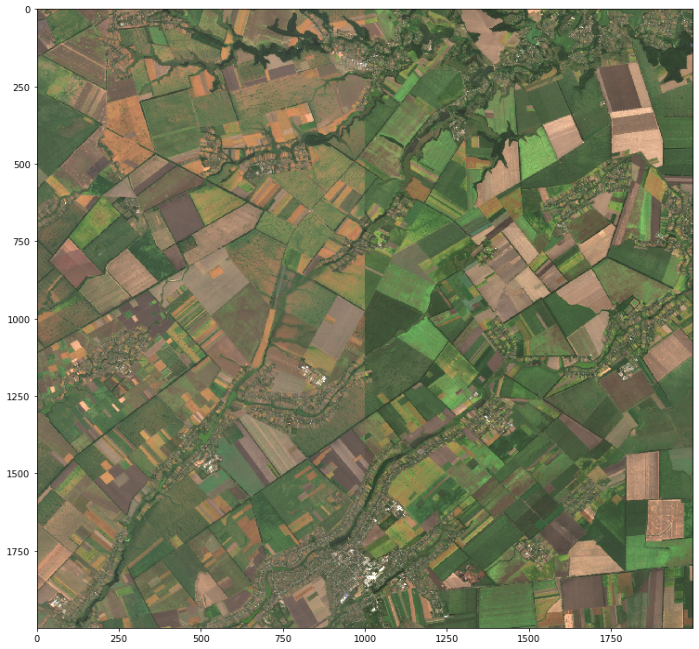
\includegraphics[width=0.6\textwidth]{images/image24}
	\caption{Знімок навчальних даних \label{fig:training-data}}
\end{figure}

Таким чином, маємо знімок, у якого ліва частина є джерелом
колірного простору, а права --- ціллю, на яку потрібно його перевести.


Дані, що були вибрані для тренування алгоритмів машинного
навчання, було взято на стику лівого і правого знімків, а саме так, щоб вони
між собою перетинались. Це дозволить зменшити контраст саме між
сусідніми регіонами знімків, тоді саме зображення матиме більш природний
колір і не буде сильного контрасту.


Варто зауважити, що якість вихідного знімка сильно залежить від
того, наскільки великий перетин навчальних даних береться, оскільки якщо взяти
доволі малий, то більш ймовірно, що результат не сильно відрізнятиметься від
оригінального знімка, тому у навчанні алгоритмів бралися 70 відсотків
області одного знімка і 30 відсотків області іншого. Це дало оптимальний результат
на виході регресійних моделей, які застосовувались для вирішення цієї
проблеми.


\textbf{NDVI}


NDVI (Normalized Difference Vegetation Index) --- нормалізований відносний
показник кількості фотосинтетичних активних біомас (зазвичай називають
вегетаційним індексом). Цей індекс будується за відбиттям від рослин
променів, що містять інфрачервоні спектральні зони. Значення індексу лежать
у діапазоні від 0,20 до 0,95. Чим зеленіший регіон для дослідження під час
вегетації, тим більше значення індексу NDVI. Таким чином, NDVI --- це
індекс, за яким можна робити висновки про розвиток зеленої зони на
супутникових знімках.

Найбільш поширене використання NDVI --- оцінка росту культур. За картою
NDVI можна оцінити територію, а саме побачити, як добре сходить
врожай, та відстежувати посуху. Для візуальної оцінки цього індексу
користуються колірною шкалою: якщо значення менше 0.25, то регіон матиме
сірий колір. Відповідно, якщо значення вище, то говорять про середній чи
нормальний розвиток тієї чи іншої культури. Результуючу інформацію
потрібно вміти аналізувати, оскільки культури сходять по-різному і на
різних часових проміжках.

У цій роботі індекс NDVI застосовується як фактор, що покращує якість
регресійних моделей, а також як елемент для оцінки точності застосування того
чи іншого алгоритму. Тому перед дослідженням до звичайного 4-канального
композиту додається ще один, а саме NDVI. Це хоч і вплинуло на швидкість
обробки методів машинного навчання, але покращило якість результуючого
знімка.

\begin{equation}
	NDVI = (Blue - Red)/(Blue + Red),
\end{equation}

де Blue --- синій, Red --- червоний
канали.

\textbf{Intensity}

Також для підвищення точності було додано 6-й канал світлості знімка,
що обчислюється за формулою:

\begin{equation}
	I = (0.42*Blue + 0.98*Green + 0.6*Red + NIR)/3
\end{equation}
